\documentclass[11pt,a4paper]{article}
\usepackage[margin=2.4cm]{geometry}
\usepackage{amsmath,amssymb,booktabs,graphicx,hyperref}
\newcommand{\avg}[1]{\{\!\{#1\}\!\}}
\newcommand{\jump}[1]{[\![#1]\!]}
\newcommand{\dt}{\Delta t}
\newcommand{\code}[1]{\texttt{#1}}
\title{The DG split-explicit algorithm:\\pressure as additional variable, MIS with the small step S2,\\contravariant momenta and the column solve by static condensation}
\author{MultiRate notes}
\date{\today}
\begin{document}
\maketitle

\begin{abstract}
The favoured algorithm for the 2D DGSEM on a terrain-following grid. The pressure is an additional prognostic variable (dry
and moist air), the operator is split into a frozen fast part, linear in the evolving state, and a slow part. A MIS step
integrates the fast part in every stage with the small step S2 (Störmer--Verlet, vertical part implicit). In the fast solver the
momenta are the contravariant ones; the column system contains the thermodynamic variables and the vertical contravariant
momentum and is solved by static condensation onto the interface momenta of the vertical faces.
\end{abstract}

\section{Equations}
Dry air, $q=(\rho,\ m=\rho\mathbf u,\ \Theta=\rho\theta)$ and the pressure $p$:
\[
\rho_t+\nabla\cdot m=0,\qquad m_t+\nabla\cdot(m\otimes\mathbf u)+\nabla p=-\rho g\,\mathbf e_z,\qquad \Theta_t+\nabla\cdot(\theta m)=0,\qquad
p_t=\frac{\partial p}{\partial\Theta}\,\Theta_t ,
\]
$p=p_0(R\Theta/p_0)^\gamma$. Moist air (Bryan \& Fritsch), $\Theta=\rho\theta_\rho$, vapour $V=\rho q_v$ and condensate $C=\rho q_c$:
\[
\Theta_t+\nabla\cdot(\theta_\rho m)=Q_\Theta,\qquad V_t+\nabla\cdot(q_vm)=-S_c,\qquad C_t+\nabla\cdot(q_cm)=S_c,\qquad
p_t=a\,\rho_t+b\,\Theta_t+c\,V_t+d\,C_t+Q_p,
\]
$(a,b,c,d)=\partial p/\partial(\rho,\Theta,V,C)$ of the moist equation of state. The phase change is a relaxation without saturation adjustment,
$S_c=-\varphi_{\rm FB}(\rho_{vs}(T)-\rho_v,\rho_c)/\tau$, $\varphi_{\rm FB}(x,y)=\tfrac12(x+y-\sqrt{x^2+y^2})$, with the latent heating
$Q_\Theta=(\partial\Theta/\partial\rho_c)S_c$ and $Q_p=(\partial p/\partial\rho_c)S_c$ along the isochoric phase change. No background state is subtracted.

\section{Spatial discretization}
Terrain-following coordinates $(\xi,\eta)$ (Gal-Chen), elements of tensor LGL nodes of degree $P$, collocated quadrature, SBP
derivative $D$, Jacobian $J$ and the contravariant metric $\tilde n_\xi=J\nabla\xi=(J\xi_x,J\xi_z)$, $\tilde n_\eta=J\nabla\eta$ at the nodes.
\begin{itemize}
\item \emph{Volume}: flux differencing along the $\xi$ and $\eta$ node lines with two-point fluxes (mass and $\Theta$ with logarithmic
  and Stolarsky means), averaged metric, the pressure $\avg p$ in the momentum flux, gravity as the non-conservative two-point term
  $\rho_{\rm avg}\,g\,(z_b-z_a)$.
\item \emph{Faces}: LMARS in $\rho\mathbf u$ along the unit normal $n$ (from $L$ to $R$), $c$ the mean face sound speed,
  \[
  m^*=\avg{m_n}-\frac{p_R-p_L}{2c},\qquad p^*=\avg p-\frac c2\,(m_{n,R}-m_{n,L}),
  \]
  mass flux $m^*$, $\Theta$-flux $\theta_{\rm up}m^*$, tracer fluxes $q_{\rm up}m^*$, momentum flux $m^*\mathbf u_{\rm up}+p^*n$ (upwind side
  from the sign of the mass flux). Equivalently $P^*_L=p_L-c(m^*-m_{n,L})=p_R+c(m^*-m_{n,R})=P^*_R$.
\item \emph{Walls}: $m^*=0$, $p^*=p+c\,m_n$.
\end{itemize}
The pressure $p$ is a nodal unknown; the state is $[\rho,m_x,m_z,\Theta\,|\,p\,(|\,V,C)]$.

\section{Frozen split}
The semi-discrete operator is written as $N(q)=F_f(C(q),q)+S(q)$: the coefficients $C$ are frozen at a state $y$, the second argument
$z$ evolves in the fast part, which is \emph{linear} in $z$ (apart from the phase change):
\begin{itemize}
\item mass, $\Theta$ and tracer fluxes: the two-point mean divided by the nodal density times the momentum of $z$, $\theta_{\rm up}$, $q_{\rm up}$
  and the pair means of $q_v$, $q_c$ from $y$;
\item momentum: the pressure of $z$ in the volume and in $p^*$, gravity with the frozen ratio of the two-point to the arithmetic mean of $\rho$;
\item faces: LMARS with $c$ and the upwind side from $y$;
\item pressure row: $p_t=b\,\Theta_t$ (dry), $p_t=a\rho_t+b\Theta_t+cV_t+dC_t$ (moist) with $(a,b,c,d)$ from $y$;
\item phase change (moist): $S_c$, $Q_\Theta$, $Q_p$ at the live state $z$, explicit in the thermodynamic part.
\end{itemize}
The slow part $S(y)$ is the momentum advection (volume and faces). $F_f(C(q),q)+S(q)=N(q)$ where $p$ equals the equation of state;
after every MIS step $p$ is reset to the equation of state of $(\rho,\Theta,V,C)$.

\section{MIS step}
Stage $i$ of a MIS step ($\alpha_{ij}$, $\beta_{ij}$, $\gamma_{ij}$, $d_i=\sum_j\beta_{ij}$; MIS54) with the stage values $Y_j$, $\Delta Y_j=Y_{j+1}-q^n$:
\[
Z(0)=q^n+\sum_{j<i}\alpha_{ij}\Delta Y_j,\qquad
Z'=F_f(\bar C_i,Z)+\bar F_i\quad\text{on }[0,d_i\dt],\qquad Y_{i+1}=Z(d_i\dt),
\]
\[
\bar C_i=\sum_{j\le i}\frac{\beta_{ij}}{d_i}C(Y_j),\qquad \bar F_i=\sum_{j\le i}\frac{\beta_{ij}}{d_i}S(Y_j)+\sum_{j<i}\frac{\gamma_{ij}}{d_i\dt}\Delta Y_j .
\]
The fast system of a stage is integrated with $n_i$ small steps of length $h=d_i\dt/n_i$.

\section{Fast system in the contravariant momenta}
Groups $T=(\rho,\Theta,p\,[,V,C])$ and $M$. In the fast solver the momenta are replaced node by node by the contravariant ones,
\[
M=(\tilde U,\tilde W)=(\tilde n_\xi\cdot m,\ \tilde n_\eta\cdot m),\qquad M=\mathcal T m,\quad \mathcal T=\begin{pmatrix}J\xi_x&J\xi_z\\J\eta_x&J\eta_z\end{pmatrix}.
\]
With $P=\mathrm{diag}(I,\mathcal T)$ the fast operator in these variables is $\tilde J=PJ_fP^{-1}$, $J_f$ the frozen operator. It is split into
\begin{itemize}
\item the \emph{vertical} part $\tilde J^z$: the $\eta$-terms ($\eta$ volume pairs, $\eta$-faces, walls) restricted to the rows and columns of $T$ and $\tilde W$;
\item the \emph{horizontal} part $\tilde J^x=\tilde J-\tilde J^z$: the $\xi$-terms and every term with $\tilde U$ (in particular the metric force $\tilde n_\xi\cdot\tilde n_\eta\,\partial_\eta p$ on $\tilde U$).
\end{itemize}
In the notation of \code{docs/fast\_2d}:
\[
T_t=A_T^xM+A_T^zM+D_T^xT+D_T^zT+f_T,\qquad M_t=A_M^xT+A_M^zT+D_M^xM+D_M^zM+f_M,
\]
$A^z$, $D^z$ the blocks of $\tilde J^z$: $A_T^z$ ($\tilde W\to T$) the vertical mass flux, $A_M^z$ ($T\to\tilde W$) the vertical pressure force and gravity,
$D_T^z$ the pressure jump of $m^*$ and $D_M^z$ the momentum jump of $p^*$ on the $\eta$-faces, the wall term. The vertical operators couple only the
nodes of one node column (fixed $\xi$-line index) and only $T$ with $\tilde W$. On a flat grid $\mathcal T$ is diagonal and $(\tilde U,\tilde W)$ are
$(m_x,m_z)$ up to the metric factors.

\section{The small step S2}\label{sec:s2}
Störmer--Verlet with the vertical part implicit (Verwer's component splitting), off-centring $\beta=(1+\varepsilon)/2$ of the vertical force:
\begin{enumerate}
\item $T^{1/2}=T^0+\tfrac h2\big(A_T^xM^0+D_T^xT^0+f_T\big)+\tfrac h2\big(A_T^zM^0+D_T^zT^0\big)$
\item $M^1=M^0+h\big(A_M^x\tilde T^{1/2}+D_M^xM^0+f_M\big)+h\big[(1-\beta)\big(A_M^zT^0+D_M^zM^0\big)+\beta\big(A_M^zT^1+D_M^zM^1\big)\big]$
\item $T^1=T^{1/2}+\tfrac h2\big(A_T^xM^1+D_T^xT^{1/2}+f_T\big)+\tfrac h2\big(A_T^zM^1+D_T^zT^1\big)$
\end{enumerate}
$\tilde T^{1/2}=T^{1/2}$, or with divergence damping $\tilde T^{1/2}=T^{1/2}+\gamma_d(T^{1/2}-T^{1/2}_{\rm prev})$ in the horizontal pressure force.
$D_M^x$ is explicit. The phase change (moist) is part of the thermodynamic tendency of stages 1 and 3. The horizontal part of stage 2,
\[
\tilde U^1=\tilde U^0+h\big(A_M^x\tilde T^{1/2}+D_M^xM^0+f_{\tilde U}\big),
\]
is explicit; with it the horizontal part of stage 3, $T^*=T^{1/2}+\tfrac h2(A_T^xM^1+D_T^xT^{1/2}+f_T)$, is explicit as well. Stages 2 and 3 are
coupled only through the vertical terms:
\[
\begin{pmatrix}I-\tfrac h2D_T^z&-\tfrac h2A_T^z\\-\beta h\,A_M^z&I-\beta h\,D_M^z\end{pmatrix}\begin{pmatrix}T^1\\\tilde W^1\end{pmatrix}=\begin{pmatrix}T^*\\\tilde W^*\end{pmatrix},\qquad
\tilde W^*=\tilde W^0+hf_{\tilde W}+(1-\beta)h\big(A_M^zT^0+D_M^z\tilde W^0\big)+h\big(A_M^x\tilde T^{1/2}+D_M^xM^0\big)_{\tilde W},
\]
one system per node column. In the code the horizontal part of stage 3 is evaluated before the solve, with $M^1$ predicted by the
momentum rows of the column system with $T$ frozen at $T^*$,
\[
\hat{\tilde W}=\tilde W^*+\beta h\,(I-\beta h\,D_M^z)^{-1}\big(A_M^zT^*+D_M^z\tilde W^*\big)
\]
($D_M^z$ couples only the two nodes of an $\eta$-face; $A_T^x$ sees $\tilde W$ only through the averaged metric of the $\xi$ volume pairs);
the half step after the solve is evaluated with the new values. The third stage of a small step and the first of the next are combined (the
horizontal self-coupling evaluated anew). In stage 2 the horizontal part acts on $M^0$, the explicit vertical force $(1-\beta)h(\dots)$ is added
after it. The small step is limited by the explicit horizontal part only.

\paragraph{Rest state.} If the spatial operator is balanced, $N(q^*)=0$ with $M^*=0$ (the isothermal atmosphere with the logarithmic density
mean in the gravity term, the constant-$\theta$ one with the Stolarsky mean, Artiano et al.), then $\tilde W^*=-\beta h\,A_M^zT^*$ (the horizontal
and the explicit vertical force), so $\hat{\tilde W}=0$, $T^*=T^0$, and the column solve returns $T^1=T^0$, $M^1=0$: S2 and the MIS step keep
$q^*$ on terrain to round-off. With $D_M^xM$ evaluated at $M^0+(1-\beta)h(\dots)$, or with the explicit predictor
$\tilde W^*+\beta h(A_M^zT^*+D_M^z\tilde W^*)$, they do not (drift $O(h^2)$ per small step).

\section{Column solve by static condensation}
In a node column with the elements $K=1,\dots,N$ and the interior $\eta$-faces $f=1,\dots,N-1$ an auxiliary unknown, the interface momentum
$\hat M_f=\tilde n_\eta\cdot m^*$ of the face node, is introduced with the exact constraint
\[
\hat M_f=\avg{\tilde W}-|\tilde n_\eta|\frac{p_R-p_L}{2c}\qquad(\Leftrightarrow P^*_L=P^*_R).
\]
Since $p^*=P^*=p_{\rm in}-c(m^*_\nu-m_{\nu,\rm in})$, every face term of an element is written with its own values and $\hat M$:
\[
\rho_t\ni-\sigma(\hat M_\nu-\tilde W_{\nu,\rm in}),\quad \Theta_t\ni-\sigma(\theta_{\rm up}\hat M_\nu-\theta\,\tilde W_{\nu,\rm in}),\quad
V_t,C_t\ \text{alike with }q_{\rm up},\quad \tilde W_t\ni\sigma c\,|\tilde n_\eta|\,(\hat M_\nu-\tilde W_{\nu,\rm in}),
\]
($\sigma=1/(J\,w_{\rm end})$ the lifting factor, $\nu$ the outward side, $p_t$ through its coefficients); the face terms contain no pressure. With $Z_K=(T_K,\tilde W_K)$ the column system becomes
\[
E_KZ_K-B_K\hat M=R_K\quad(K=1,\dots,N),\qquad \hat M=\sum_KG_KZ_K,
\]
$E_K=I-\Delta J_{KK}$, $B_K=\Delta J_{K\hat M}$, $\Delta=\mathrm{diag}(\tfrac h2\text{ on }T,\ \beta h\text{ on }\tilde W)$, $G_K$ the constraint. Different elements
are coupled only through $\hat M$. The solve:
\begin{enumerate}
\item $Z_K=y_K+W_K\hat M$, $y_K=E_K^{-1}R_K$, $W_K=E_K^{-1}B_K$ (one dense system per element);
\item $\big(I-\sum_KG_KW_K\big)\hat M=\sum_KG_Ky_K$, tridiagonal of size $N-1$;
\item $Z_K=y_K+W_K\hat M$.
\end{enumerate}
$\hat M$ is not kept; the result is the solution of the column system. The factorization is done once per stage and weight pair. Since
element $K$ touches only the faces $K-1$ and $K$, $W_K$ has two columns and $G_K$ two rows; $E_K^{-1}$ is stored as a dense inverse, so
a solve costs per element one product with $E_K^{-1}$ and two with $W_K$, $G_K$, per column one tridiagonal solve.

\section{Examples}
All runs: MIS54, S2 (\code{fast = :cs}), $\varepsilon=0.1$, \code{lmars = :momentum}, $h$ at the explicit horizontal limit.

\begin{figure}[h]\centering
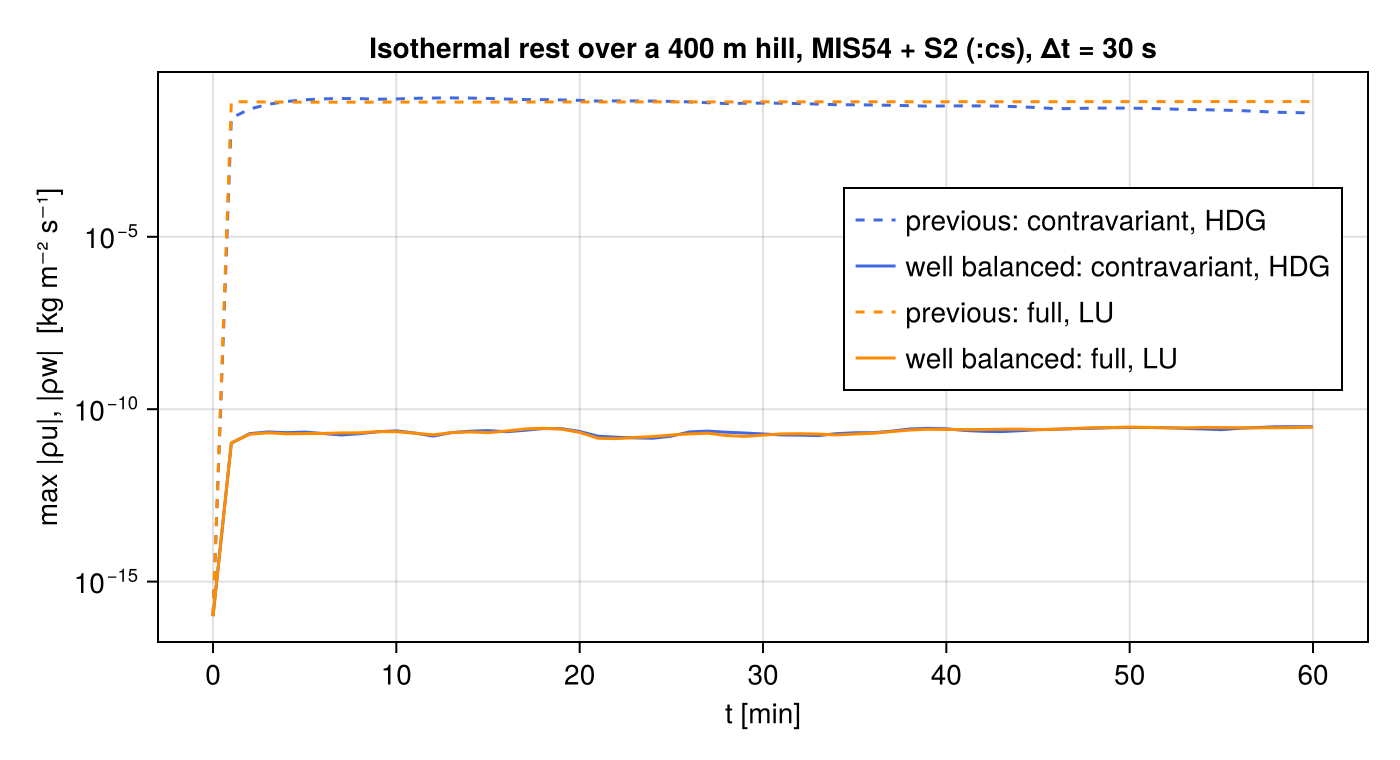
\includegraphics[width=0.75\textwidth]{rest_drift.png}
\caption{Isothermal atmosphere ($T=250$\,K) at rest over a 400\,m hill (80\,km$\times$10\,km, $8\times4$ elements, $P=3$), $\dt=30$\,s,
24 small steps. Maximum of the momenta; dashed: S2 with $D_M^x$ acting on $M^0+(1-\beta)h(\dots)$ and the explicit predictor (commit
\code{a149165}), solid: the form of Section~\ref{sec:s2}. Blue: contravariant momenta, HDG; orange: \code{vsplit = :full}, LU.}
\end{figure}

\begin{figure}[h]\centering
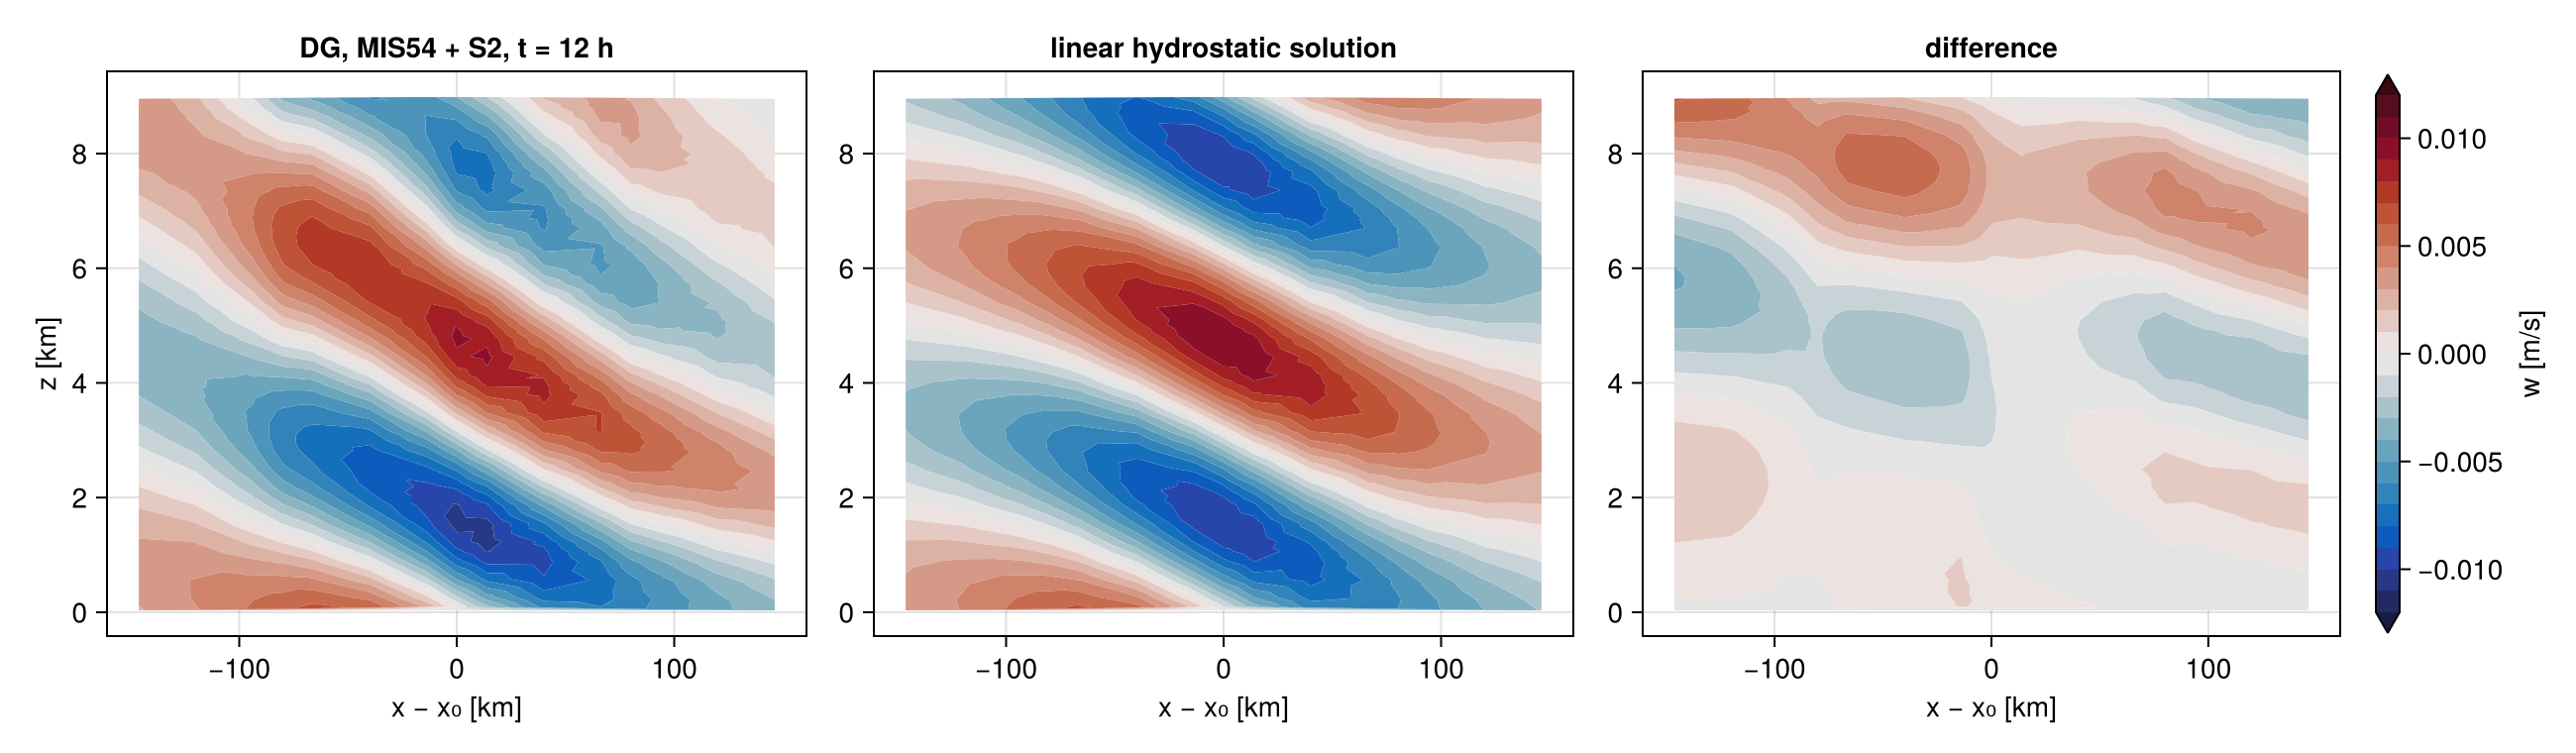
\includegraphics[width=\textwidth]{a100_w.png}
\caption{Hydrostatic flow over the Agnesi hill, $a=100$\,km, $h_0=100$\,m, $U=10$\,m/s, $N=0.01$\,s$^{-1}$, $50\times16$ elements, $P=4$,
sponge above 9\,km, $\dt=300$\,s, 22 small steps; contravariant momenta, HDG. Vertical velocity at $t=12$\,h, the linear hydrostatic
steady solution and the difference. One MIS step costs 1.6\,s (HDG) and 1.7\,s (LU).}
\end{figure}

\begin{figure}[h]\centering
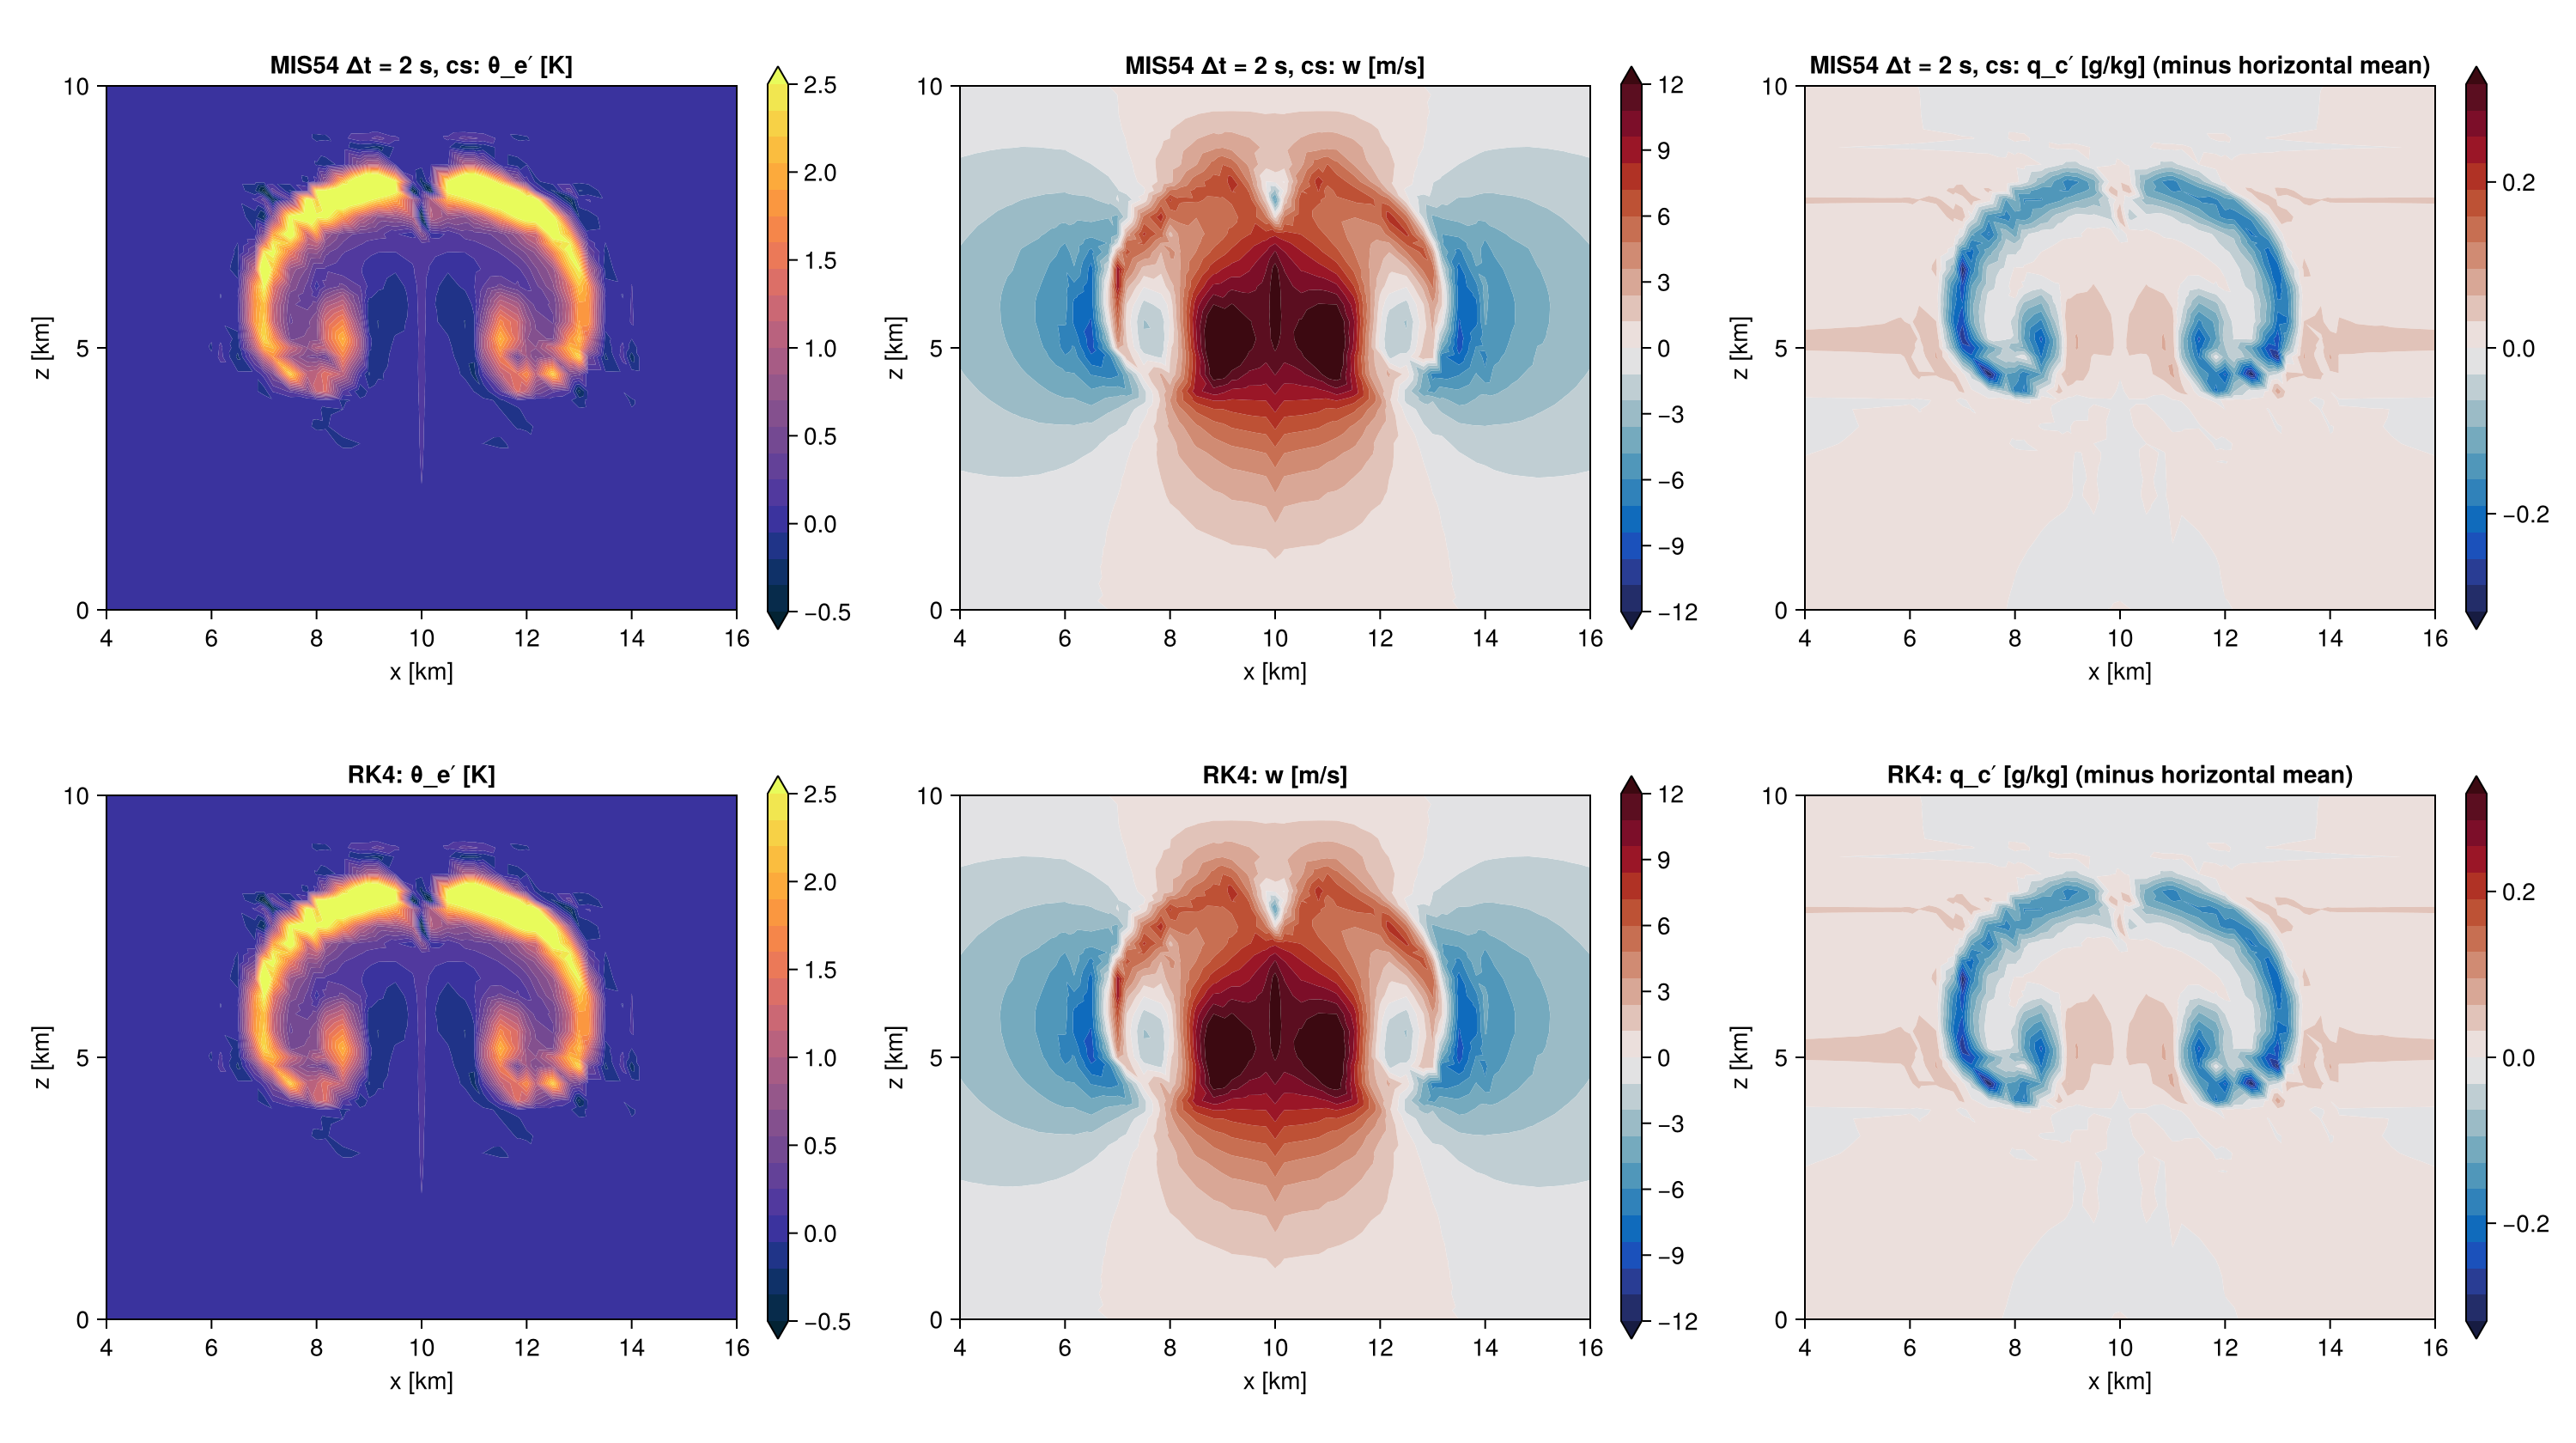
\includegraphics[width=\textwidth]{moist_bubble.png}
\caption{Moist bubble (saturated neutral atmosphere, $\theta_e=320$\,K, $r_t=0.02$, 20\,km$\times$10\,km, $20\times10$ elements, $P=4$) at
$t=1000$\,s, moist pressure model with HDG; top: MIS54 with $\dt=2$\,s, bottom: RK4 reference.}
\end{figure}
\clearpage

\section{Parameters and implementation}
\begin{center}\small
\begin{tabular}{ll}\toprule
MIS method & MIS54, $\dt$ advective \\
small step & S2 at the explicit horizontal limit, $h\le0.85\cdot0.63\,\Delta x_e/((2P+1)c)$ \\
off-centring, divergence damping & $\varepsilon=0.1$, $\gamma_d=0$--$0.1$ \\
phase change (moist) & $\tau=\tfrac12\cdot0.85\cdot0.63\,\Delta x_e/((2P+1)c_s)$, in every small step \\\bottomrule
\end{tabular}
\end{center}
\noindent\code{src/DGSEM/Euler2D/frozen\_p.jl}:
\begin{verbatim}
m = DGPressureModel(base; lmars = :momentum, vsplit = :contravariant_momentum,
                    vsolver = :hdg, hpredict = false [, moist = true, mgas, tau])
q = run_frozen(m, q0, dt, n; tab = mis_tableau(:MIS54), nsub, fast = :cs,
               offcenter = 0.1, smdiv = 0.0)
\end{verbatim}
\code{vsplit = :contravariant\_momentum}: the split of the contravariant fast operator, assembled in Cartesian variables as
$J_v=P^{-1}\tilde J^zP$, $J_h=J_f-J_v$ (the time stepper is unchanged); \code{vsolver = :hdg}: the static condensation (\code{\_hdg\_factor}),
\code{:lu} the same system by a sparse LU; \code{hpredict = false}: $D_M^x$ explicit as in stage 2. Examples: \code{examples/frozen\_dg\_cs.jl} (gravity
wave over a hill), \code{examples/sk94\_long\_channel.jl}, \code{examples/dg\_moist\_bubble.jl} (\code{FAST=cs VSOLVER=hdg DTS=2}); figures: \code{docs/dg\_algorithm/figures}.
\end{document}
